\chapter[Cosmogenic Nuclides]{Cosmogenic nuclide geochronology}
\label{sec:cosmo}

The Earth is constantly bombarded by galactic cosmic rays, which
primarily consist of protons. Many of these electrically charged
particles never reach our planet because they are deflected back into
space by the Earth's magnetic field (see Equation \ref{eq:Hev}). The
degree of `protection' provided by the magnetic field is greater at
low latitudes (where the magnetic field lines run parallel to the
surface) than at the poles (where they are perpendicular to the
surface). Thus, the cosmic ray intensity at the equator is
significantly lower than at the poles, although the average energy (or
`rigidity') of the cosmic rays is higher\footnote{At the poles, even
  low energy solar cosmic rays (which predominantly consist of
  electrons, not protons) can reach the upper atmosphere, giving rise
  to the Aurora Borealis.}\\

The primary cosmic rays which do manage to pass through the magnetic
field strongly interact with the atmosphere and form a secondary
cosmic ray `shower', which is mostly made of neutrons and muons. This
secondary cosmic ray shower is rapidly attenuated as it travels down
into the atmosphere. Only a very small fraction of the secondary
cosmic rays, which mostly consist of neutrons, reach the surface of
the Earth. These neutrons then collide with the elements that are
found in rocks and soils, such as silicon, oxygen, calcium etc. When
such an element is hit by a cosmic ray, it undergoes `spallation',
which basically means that it explodes into smaller particles. Most of
these particles are either very short lived or very common in the
Earth's crust. But some of the spallation products are very rare yet
sufficiently long lived to accumulate in measurable quantities in
terrestrial rocks. One example is $^{10}$Be, which has a half life of
1.3 million years. This is orders of magnitude shorter than the age of
the Earth. So, just like the $^{14}$C discussed in Section
\ref{sec:14C}, the existence of $^{10}$Be on our planet would be
impossible to explain without these cosmogenic production pathways. \\

The production of \emph{cosmogenic nuclides} is restricted to the
uppermost few meters below the surface. So if the concentration of the
$^{10}$Be in the surface rocks is known, and if the production rate is
known, then the exposure age of the rock can be estimated. This is
similar to measuring how long a person has been exposed to sunlight by
measuring the tan of their skin. During the 20 years or so that
cosmogenic nuclide geochronology has been around, it has truly
revolutionised various aspects of geomorphology, such as the study of
volcanoes, river incision, landslides, glaciers, sediments, and
faults.\\

\begin{table}[!ht]
\centering
\begin{tabular}{l@{~}l@{~}l@{~}l}
nuclide & half life & reaction types & target minerals \\
\hline
$^3$He & stable & spallation on O, Si & olivine, pyroxene \\
$^{21}$Ne & stable & spallation on Mg, Fe & quartz \\
$^{10}$Be & 1.36 Myr & $^{16}$O(n,4p3n)$^{10}$Be & quartz \\
~ & ~ & $^{28}$Si(n,x)$^{10}$Be & ~ \\
$^{26}$Al & 717 kyr & $^{28}$Si(n,p2n)$^{26}$Al & quartz\\
$^{36}$Cl & 301 kyr & $^{40}$Ca(n,2n3p)$^{36}$Cl & calcite, plagioclase\\
~ & ~ & $^{39}$K($\mu^-$,p2n)$^{36}$Cl & ~ \\
~ & ~ & $^{40}$Ca($\mu^-$,$\alpha$)$^{36}$Cl & ~ \\
~ & ~ & $^{35}$Cl(n,$\mu$)$^{36}$Cl & ~ \\
$^{14}$C & 5730 yr & $^{16}$O(n,2pn)$^{14}$C & quartz\\
\end{tabular}
\caption{Commonly used terrestrial cosmogenic nuclides.}
\label{tab:cosmo}
\end{table}

Table \ref{tab:cosmo} lists the most commonly used cosmogenic
nuclides. What all these isotopes have in common is that they are
normally absent from rocks that are shielded from cosmic rays. They
belong to two categories. There are the cosmogenic noble gases, which
are stable, and the cosmogenic radionuclides, which are
radioactive. Each of these have different applications.

\section{Stable nuclides}

In the simplest case of a stable nuclide in the absence of erosion,
its concentration increases linearly with time (t). So if we measure
the concentration (N) in atoms per gram of, say, quartz, and if we
know the production rate (P), in atoms per gram per year, then we can
simply calculate the age by dividing the concentration by the
production rate:

\begin{equation}
t = \frac{N}{P}
\label{eq:cosmo-exposure}
\end{equation}

Next, consider the situation of a stable nuclide and a rock surface
that is in steady state erosion. To understand this situation, it is
useful to imagine one in the place of a rock particle under an eroding
surface. As the particle approaches the surface, it sees an
exponentially increasing cosmic ray intensity and cosmogenic nuclide
production rate. So in the case of an eroding surface, the cosmogenic
nuclide content can be used not to measure an exposure age, but an
erosion rate ($\epsilon$). $\epsilon$ is a simple function of the
production rate $P$ and the concentration $N$, multiplied by a factor
$\Lambda/\rho$, where $\rho$ is the rock density and $\Lambda$ is the
attenuation length ($\sim$160 g/cm$^{-2}$).  This factor quantifies
how rapidly the cosmic ray intensity decreases with depth in the rock:

\begin{equation}
\epsilon = \frac{\Lambda}{\rho} \frac{P}{N}
\label{eq:cosmo-erosion}
\end{equation}

\section{Radionuclides}

Let us now move on to a cosmogenic radionuclide in a surface that
undergoes no erosion. Initially, the concentration of the nuclide
increases almost linearly with time, but after a while, some of these
nuclides are lost due to radioactive decay. Eventually, after five or
so half lives, a saturation point is reached at which the production
rate is balanced by the decay rate. This provides a hard upper limit
of the exposure ages that can be measured with cosmogenic
radionuclides. The age equation is again a function of $P$ and $N$,
but with the addition of a logarithm and the radioactive decay
constant $\lambda$:

\begin{equation}
t = -\frac{1}{\lambda} \ln\left(1-\frac{N\lambda}{P}\right)
\label{eq:cosmo-radioexposure}
\end{equation}

Finally, here is the full ingrowth equation in the general case of a
cosmogenic radionuclide with a finite exposure age that also undergoes
erosion:

\begin{equation}
N = \frac{P}{\lambda + \rho\epsilon/\Lambda}
\left(1-e^{-(\lambda+\rho\epsilon/\Lambda)t}\right) e^{-\lambda\tau}
\label{eq:cosmo-N}
\end{equation}

with:\\

$N$ = concentration (at/g)\\
\indent $P$ = production rate (at/g/yr)\\
\indent $\lambda$ = decay constant (yr$^{-1}$)\\
\indent $\Lambda$ = attenuation length (g/cm$^{-2}$)\\
\indent $\rho$ = density (g/cm$^{-3}$)\\
\indent $\epsilon$ = erosion rate (cm/yr)\\
\indent $t$ = exposure age (yr)\\
\indent $\tau$ = burial age (yr)\\

There is one additional parameter, $\tau$, which is the \emph{burial
  age}, which will be discussed in Section \ref{sec:banana}. The
important thing to note here is that there is one equation but three
unknowns, the exposure age $t$, the erosion rate $\epsilon$, and the
burial age $\tau$. So in order to solve this equation, two assumptions
are needed. For example, if we assume zero burial ($\tau$ = 0) and
zero erosion ($\epsilon$ = 0), then we calculate the exposure age
($t$). Alternatively, we can assume zero burial and an infinite
exposure age ($\tau$ = 0, t=$\infty$) and calculate the steady state
erosion rate ($\epsilon$). The only way to avoid making such
assumptions and simultaneously determining both the erosion rate and
the exposure age is to measure two nuclides with different half
lives. The most common examples of such paired measurements are
$^{10}$Be/$^{26}$Al and $^{10}$Be/$^{21}$Ne. A convenient method to
plot and interpret such datasets is the two nuclide diagram or `banana
plot'.

\section{The `Banana Plot'}
\label{sec:banana}

When we plot the $^{26}$Al/$^{10}$Be-ratio against the $^{10}$Be
concentration, we obtain the diagram shown in Figure \ref{fig:banana}.
Each part of this diagram has its own applications, which will be
briefly summarised next.\\

\begin{figure}[!ht]
  \centering
  \ifpdf
  \def\svgwidth{.8\textwidth}
  ~~(i)~\input{AlBe.pdf_tex}\\
  \def\svgwidth{.8\textwidth}
  (ii)\input{NeBe.pdf_tex}
  \else
  (i)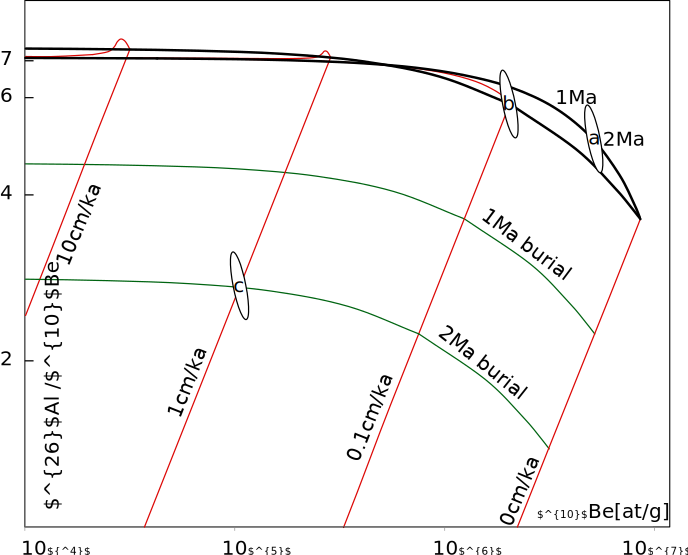
\includegraphics[width=5cm]{../figures/AlBe.png}
  (ii)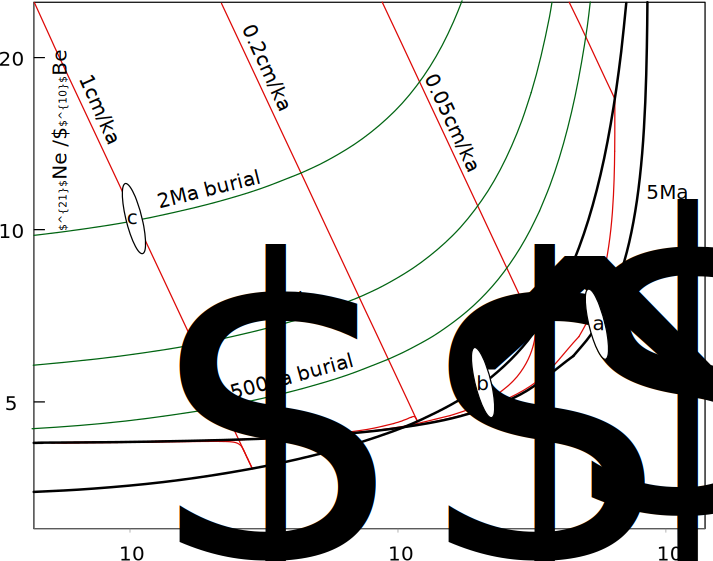
\includegraphics[width=5cm]{../figures/NeBe.png}
  \fi
  \caption{$^{10}$Be/$^{26}$Al (i) and $^{21}$Ne/$^{10}$Be (ii) two
    nuclide (`banana') plots. Sample a has undergone a simple exposure
    history with $t$ = 2Ma, $\epsilon = 0$ and $\tau$ = 0, sample b has
    undergone steady-state erosion at $\epsilon$ = 0.1cm/kyr (t =
    $\infty$ and $\tau$ = 0), whereas sample c has experience a complex
    exposure history. Assuming steady-state erosion prior to burial, the
    data are compatible with $\epsilon$ = 1 cm/kyr followed by 2 Myr of
    burial. The ellipses mark the 95\% confidence bounds for the
    analytical uncertainties (see Section \ref{ch:error-propagation}).}
  \label{fig:banana}
\end{figure}

First consider a sample that plots on the upper line of the
diagram. This is the so-called \emph{zero erosion line}, which groups
all samples that can be used for proper exposure dating. So if a
sample plots on this line, we have effectively verified the assumption
that $\epsilon=0$.  The most important example of studies which
require samples that plot on the zero erosion line are exposure dating
studies of glacial retreat. When glacial striations can be observed on
rock surfaces, this indicates that erosion has been negligible. All
those surfaces should plot on the zero erosion line of the banana
plot.\\

The next line down groups all the samples that are in an erosional
steady state and that, in principle have an infinite exposure age
($t=\infty$), which effectively means an exposure age that is greater
than five times the half lives of both nuclides.  Although erosion
studies can be performed in bedrock, they are actually most commonly
done on sediments. The motivation for this is as follows. Consider a
landscape that is in an erosional steady state and that is irradiated
by cosmic rays. Cosmogenic nuclides such as $^{10}$Be accumulate in
the first 2m or so below the surface. These rocks are removed and
transported down the drainage network, carrying the cosmogenic nuclide
signal with them. By measuring the $^{10}$Be content of a single
sample of river sediment, the average erosion rate of the entire
catchment can be calculated.\\

So the upper line of the $^{10}$Be/$^{26}$Al banana plot is the zero
erosion line, the lower line is the steady state erosion line, and the
area between them is called the \emph{steady state erosion island} (or
\emph{banana}).  Above the erosion island is the `forbidden zone' of
physically impossible cosmogenic nuclide compositions. Samples
plotting in this area are likely to suffer from methodological or
analytical errors. The large area below the erosion island is the zone
of \emph{complex exposure histories}, in which we can find samples
that have undergone at least one phase of burial. For example,
consider a river sediment derived from a catchment that is in an
erosional steady state (e.g., $\epsilon$ = 0.1cm/kyr) and has
accumulated a measurable amount of cosmogenic $^{10}$Be and
$^{26}$Al. Suppose that this sediment is washed into a cave.  The roof
of the cave will shield the sample from cosmic rays, so that the
production of $^{10}$Be and $^{26}$Al stops, but their radioactive
decay continues. So with time, the sample will move down a line on the
banana plot. The burial age can be calculated from the distance of the
sample below the steady state erosion island.  Obviously, the most
common application of burial dating is the dating of cave
sediments. By measuring the age of different cave levels in the walls
of a river canyon, it is possible to determine the rate of canyon
incision.

\section{Scaling models}
\label{sec:scaling}

So far in this Chapter, we have assumed that the cosmogenic nuclide
production rate $P$ is known. In reality, however, this is only the
case for a handful of locations (`calibration sites') in the world,
where the exposure history of rocks is known through independent means
(e.g. by $^{14}$C dating of organic matter or $^{40}$Ar/$^{39}$Ar
dating of lava flows. These production rates are only valid for the
specific conditions (latitude, elevation, age) of each particular
calibration site. To apply the cosmogenic nuclide method to other
field settings, the production rates must be scaled to a common
reference at sea level and high latitude (SLHL). Up to 20\%
uncertainty is associated with this scaling, constituting the bulk of
cosmogenic nuclide age uncertainty.\\

Although several efforts have been made to directly measure production
rate scaling with latitude and elevation using artificial H$_{2}$O and
SiO$_2$ targets, all currently used scaling models are based on
neutron monitor surveys. The oldest and still most widely used scaling
model is that of Lal (1991). This model is a simple set of polynomial
equations giving the (spallogenic + muogenic) production rate relative
to SLHL as a function of geographic latitude and elevation.\\

Despite their limitations, the production rate scaling factors allow
the calculation of TCN production rates at any location on the Earth's
surface, assuming that the sample is a slab of zero thickness taken
from a horizontal planar surface. If these assumption are not
fulfilled, the SLHL production rates must be multiplied by a second
set of correction factors, quantifying the extent to which the cosmic
rays were blocked by topographic obstructions, snow cover, and the
thickness of the sample (`self shielding').
